\documentclass[11pt,a4paper]{article}

% Compilar con: tectonic funciones_pars_dinamicos.tex
\usepackage{fontspec}
\usepackage{amsmath,amssymb}
\usepackage[margin=2.0cm]{geometry}
\usepackage{xcolor}
\usepackage{booktabs}
\usepackage{underscore}
\usepackage{titlesec}
\usepackage{pgfplots}
\pgfplotsset{compat=1.18}
\usepackage[hidelinks]{hyperref}

\definecolor{cazul}{HTML}{2C5F8A}
\definecolor{cnaranja}{HTML}{C1660A}
\definecolor{cgris}{HTML}{5B6770}
\definecolor{serieA}{HTML}{2A78D6}
\definecolor{serieB}{HTML}{EB6834}
\definecolor{tinta2}{HTML}{52514E}

\emergencystretch=3em
\setlength{\parindent}{0pt}
\setlength{\parskip}{4pt}
\titleformat{\section}{\normalfont\Large\bfseries\color{cazul}}{}{0em}{}
\titlespacing*{\section}{0pt}{0pt}{4pt}
\newcommand{\code}[1]{\texttt{\small #1}}

\pgfplotsset{
  estilo/.style={
    width=\linewidth, height=4.6cm,
    axis line style={tinta2!60}, tick style={tinta2!60},
    major grid style={gray!18}, grid=major,
    tick label style={font=\footnotesize}, label style={font=\footnotesize, color=tinta2},
    legend style={font=\scriptsize, draw=none, fill=white, fill opacity=0.8, text opacity=1},
    xlabel={$\tilde s_t$ (índice de estado suavizado)}, domain=-3:3, samples=80,
  },
}

\begin{document}
\pagestyle{plain}
\section*{Funciones de los parámetros dinámicos de Alginvesting}
{\color{cgris}\small Estado al cierre de la Fase 2 (X5\_Q4), 2026-11-02. Siete parámetros, calibrados por activo sobre las tablas de estado de Q1.
Un buen ajuste mide qué tan bien la curva reproduce su propio target por percentil causal; no es evidencia de que el parámetro dinámico mejore el retorno (eso es Q5).}

\subsection*{Forma común}
Para un parámetro $P$ con $k$ variables explicativas $x_{1,t},\dots,x_{k,t}$ (algunas con signo invertido para que la pendiente esperada sea positiva):
\[
z_{i,t}=\frac{x_{i,t}-\mu_i}{\sigma_i},\qquad
s_t=\sum_{i=1}^{k}w_i\,z_{i,t},\quad \sum_i w_i=1,\qquad
\tilde s_t=\alpha\,s_t+(1-\alpha)\,\tilde s_{t-1},\ \ \alpha=\frac{2}{12+1}
\]
\[
\hat P_t=\text{piso}+\frac{\text{techo}-\text{piso}}{1+\exp\!\big(-\text{pendiente}\,(\tilde s_t-\text{punto\_medio})\big)},
\qquad \text{elasticidad}=\frac{\text{pendiente}\,(\text{techo}-\text{piso})}{4}.
\]
$\mu_i,\sigma_i$ son media y desviación estándar de la variable sobre todo el histórico de calibración (desde 2022-01-01), congeladas. \code{punto\_medio} y \code{pendiente} se ajustan por mínimos cuadrados (\code{curve\_fit}) contra $y^*_t=\text{piso}+(\text{techo}-\text{piso})\,q_t$, donde $q_t$ es el percentil causal de $\tilde s_t$ (usa solo el pasado de cada barra).

\subsection*{Pisos y techos}
Viven en \code{scripts/config\_smart.py}, separados en cripto (BTCUSD, ETHUSD) y acciones, y se pueden mover sin tocar código.

\begin{center}\small
\begin{tabular}{lcccc}
\toprule
Parámetro & Piso cripto & Techo cripto & Piso acción & Techo acción \\
\midrule
\code{N} & 50 & 200 & 40 & 180 \\
\code{A} & 2 & 20 & 2 & 20 \\
\code{factor\_B} & 0.2 & 0.7 & 0.2 & 0.7 \\
\code{K} & 0.5 & 2 & 0.5 & 2 \\
\code{N\_EXP} & 0.5 & 3 & 0.5 & 3 \\
\code{LAMBDA} & 0.05 & 0.5 & 0.05 & 0.5 \\
\code{PERDIDA\_MAX} & 100 & 300 & 100 & 300 \\
\bottomrule
\end{tabular}
\end{center}
\newpage
\section*{$N$ --- cantidad de soportes activos}

\textbf{Qué controla.} Cantidad de soportes que X1 mantiene activos por activo (\code{n\_sizes\_ejecucion}). Más $N$ reparte el capital en más niveles, más finos y más chicos; menos $N$ lo concentra.

\textbf{Hipótesis.} Drawdown sano, volatilidad baja y subidas más variables que las bajadas $\rightarrow$ $N$ alto. Drawdown profundo, volatilidad alta y bajadas más variables $\rightarrow$ $N$ bajo.

\textbf{Variables} (velas H1):
\begin{itemize}\setlength{\itemsep}{1pt}\setlength{\topsep}{1pt}
\item $x_1=\text{drawdown}_{30d}=(C_t-M_t)/M_t$, con $M_t=\max_{i=t-719..t}C_i$ (30 días de velas H1).
\item $x_2=-\text{atr\_pct}$, con $\text{atr\_pct}=ATR_{14}/C_t$ (ATR de Wilder). Signo invertido: volatilidad alta baja $N$.
\item $x_3=\ln(\sigma^{\uparrow}_{30d}/\sigma^{\downarrow}_{30d})$: razón entre la desviación estándar de los retornos positivos y la de los negativos en 30 días.
\end{itemize}
Pesos fijos $[0.6,\,0.2,\,0.2]$ (decisión de Mauricio, 2026-11-02); Q5 los calibra. Suavizado: EMA causal con \code{span=12}.

\begin{center}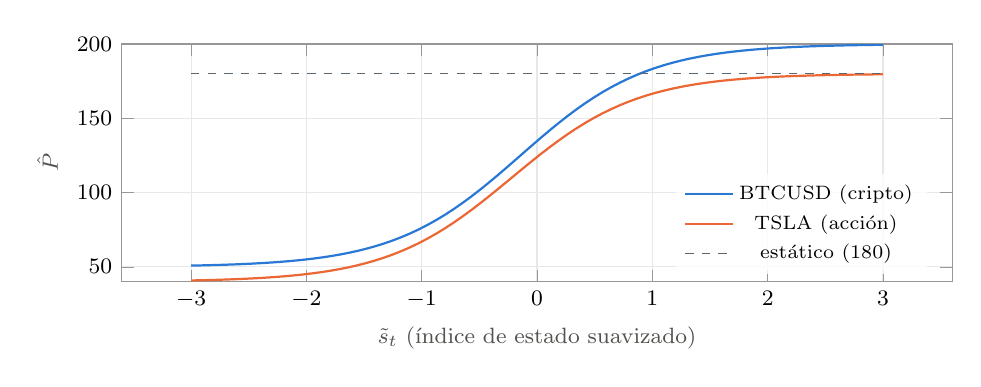
\begin{tikzpicture}\begin{axis}[estilo, ylabel={$\hat P$}, ymin=40, ymax=200, legend pos=south east]
\addplot[color=serieA, thick] {50+(200-50)/(1+exp(-1.81254*(x-(-0.143425))))};\addlegendentry{BTCUSD (cripto)}
\addplot[color=serieB, thick] {40+(180-40)/(1+exp(-1.83708*(x-(-0.220031))))};\addlegendentry{TSLA (acción)}
\addplot[color=cgris, dashed] {180};\addlegendentry{estático (180)}
\end{axis}\end{tikzpicture}\end{center}
\begin{center}\small\setlength{\tabcolsep}{5pt}
\begin{tabular}{llcccc}\toprule
Activo & Pesos $w_i$ & punto\_medio & pendiente & $R^2$ & Estático \\\midrule
BTCUSD & [0.60, 0.20, 0.20] & -0.1434 & 1.813 & 0.864 & 180 \\
ETHUSD & [0.60, 0.20, 0.20] & -0.05352 & 1.765 & 0.846 & 180 \\
TSLA & [0.60, 0.20, 0.20] & -0.22 & 1.837 & 0.869 & 180 \\
GOOGL & [0.60, 0.20, 0.20] & -0.2001 & 1.615 & 0.784 & 180 \\
NVDA & [0.60, 0.20, 0.20] & -0.3054 & 1.271 & 0.668 & 180 \\
AMZN & [0.60, 0.20, 0.20] & -0.1476 & 1.526 & 0.755 & 180 \\
MSFT & [0.60, 0.20, 0.20] & -0.1826 & 1.833 & 0.843 & 180 \\
\bottomrule\end{tabular}

\medskip
\begin{tabular}{lrrrrrr}\toprule
Activo & $\mu_1$ & $\sigma_1$ & $\mu_2$ & $\sigma_2$ & $\mu_3$ & $\sigma_3$ \\\midrule
BTCUSD & -0.08866 & 0.07642 & -0.007148 & 0.003491 & -0.02265 & 0.1636 \\
ETHUSD & -0.1247 & 0.1018 & -0.009463 & 0.004752 & -0.03965 & 0.1939 \\
TSLA & -0.1896 & 0.1303 & -0.01385 & 0.004534 & -0.007012 & 0.1594 \\
GOOGL & -0.1011 & 0.08165 & -0.008468 & 0.002434 & 0.06248 & 0.2487 \\
NVDA & -0.1192 & 0.1113 & -0.01195 & 0.004398 & 0.03585 & 0.2848 \\
AMZN & -0.1055 & 0.09702 & -0.008565 & 0.003272 & 0.05853 & 0.3092 \\
MSFT & -0.08644 & 0.06644 & -0.0067 & 0.002345 & 0.03845 & 0.2933 \\
\bottomrule\end{tabular}\end{center}
\textbf{Lectura.} El estático (180) coincide con el techo de las acciones $(40,180)$, así que el $N_t$ dinámico nunca lo supera en acciones. Mejores ajustes en cripto ($R^2\approx0.85$) que en NVDA, AMZN y GOOGL ($0.67$--$0.78$).
\newpage
\section*{$A$ --- ganancia mínima para activar el trailing / distancia de la orden en espera}

\textbf{Qué controla.} USD de ganancia mínima ($A=(P_0-P_i)\cdot L$) para poner el primer stop ganador, y a la vez filtro de distancia al crear órdenes en espera. Escala con el lotaje real de cada posición.

\textbf{Hipótesis.} Volatilidad alta y subidas más variables que las bajadas $\rightarrow$ $A$ alto (exigir más recorrido antes de operar). Pendiente positiva en las dos variables, sin invertir.

\textbf{Variables} (velas H1):
\begin{itemize}\setlength{\itemsep}{1pt}\setlength{\topsep}{1pt}
\item $x_1=\text{atr\_pct}_t=ATR_{14,t}/C_t$ (ATR de Wilder, $\alpha=1/14$).
\item $x_2=\ln(\sigma^{\uparrow}_{30d}/\sigma^{\downarrow}_{30d})$ (misma que en $N$).
\end{itemize}
Pesos fijos $[0.7,\,0.3]$ (decisión de Mauricio, 2026-11-02); Q5 los calibra. Suavizado: EMA causal con \code{span=12}.

\begin{center}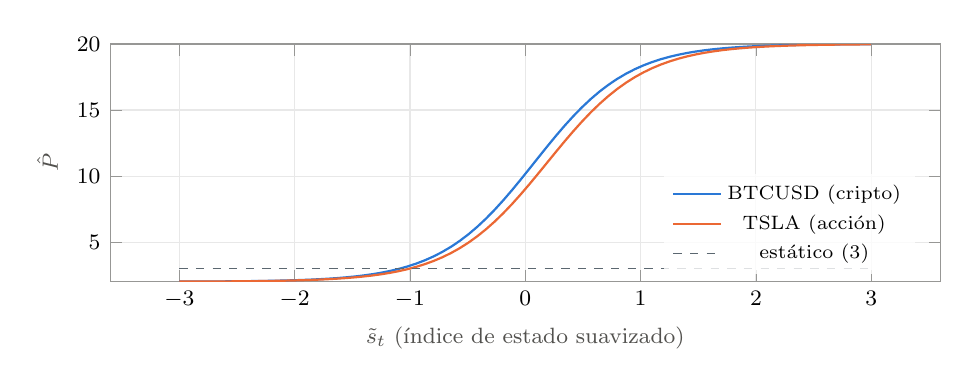
\begin{tikzpicture}\begin{axis}[estilo, ylabel={$\hat P$}, ymin=2, ymax=20, legend pos=south east]
\addplot[color=serieA, thick] {2+(20-2)/(1+exp(-2.44166*(x-(0.0762676))))};\addlegendentry{BTCUSD (cripto)}
\addplot[color=serieB, thick] {2+(20-2)/(1+exp(-2.38818*(x-(0.18786))))};\addlegendentry{TSLA (acción)}
\addplot[color=cgris, dashed] {3};\addlegendentry{estático (3)}
\end{axis}\end{tikzpicture}\end{center}
\begin{center}\small\setlength{\tabcolsep}{5pt}
\begin{tabular}{llcccc}\toprule
Activo & Pesos $w_i$ & punto\_medio & pendiente & $R^2$ & Estático \\\midrule
BTCUSD & [0.70, 0.30] & 0.07627 & 2.442 & 0.909 & 3 \\
ETHUSD & [0.70, 0.30] & -0.004387 & 2.411 & 0.901 & 3 \\
TSLA & [0.70, 0.30] & 0.1879 & 2.388 & 0.900 & 3 \\
GOOGL & [0.70, 0.30] & 0.2728 & 1.732 & 0.656 & 3 \\
NVDA & [0.70, 0.30] & 0.4865 & 1.745 & 0.727 & 3 \\
AMZN & [0.70, 0.30] & 0.4178 & 1.62 & 0.626 & 3 \\
MSFT & [0.70, 0.30] & 0.3261 & 1.772 & 0.642 & 3 \\
\bottomrule\end{tabular}

\medskip
\begin{tabular}{lrrrr}\toprule
Activo & $\mu_1$ & $\sigma_1$ & $\mu_2$ & $\sigma_2$ \\\midrule
BTCUSD & 0.007148 & 0.003491 & -0.02265 & 0.1636 \\
ETHUSD & 0.009463 & 0.004752 & -0.03965 & 0.1939 \\
TSLA & 0.01385 & 0.004534 & -0.007012 & 0.1594 \\
GOOGL & 0.008468 & 0.002434 & 0.06248 & 0.2487 \\
NVDA & 0.01195 & 0.004398 & 0.03585 & 0.2848 \\
AMZN & 0.008565 & 0.003272 & 0.05853 & 0.3092 \\
MSFT & 0.0067 & 0.002345 & 0.03845 & 0.2933 \\
\bottomrule\end{tabular}\end{center}
\textbf{Lectura.} $A$ se calibra único: no separa \code{A\_OE} de \code{A\_TRAILING} (decisión pendiente, \code{x5\_contexto\_conversacion.md} §21). El estático (3 USD) queda pegado al piso del rango, por lo que $A_t$ lo supera en 95\%--100\% de las barras.
\newpage
\section*{$\text{factor}_B$ --- holgura del trailing stop respecto de $A$}

\textbf{Qué controla.} Multiplicador adimensional con $B=\text{factor}_B\cdot A$. $B$ es la distancia monetaria entre el precio y el stop una vez activado el trailing. Factor bajo: trailing ajustado; alto: trailing holgado.

\textbf{Hipótesis.} Volatilidad alta y tendencia fuerte $\rightarrow$ $\text{factor}_B$ alto (dejar correr la posición). Mercado lateral o ruidoso $\rightarrow$ bajo o intermedio.

\textbf{Variables} (velas H1):
\begin{itemize}\setlength{\itemsep}{1pt}\setlength{\topsep}{1pt}
\item $x_1=\text{atr\_pct}_t$ (como en $A$).
\item $x_2=ADX_{14,t}$: índice de movimiento direccional promedio de Wilder; mide fuerza de tendencia sin importar el signo.
\end{itemize}
Peso $w_1$ elegido por grilla $0.1$--$0.9$ y mejor $R^2$: sale $[0.1,\,0.9]$ en los 7 activos (el ADX casi solo). Suavizado: EMA causal con \code{span=12}.

\begin{center}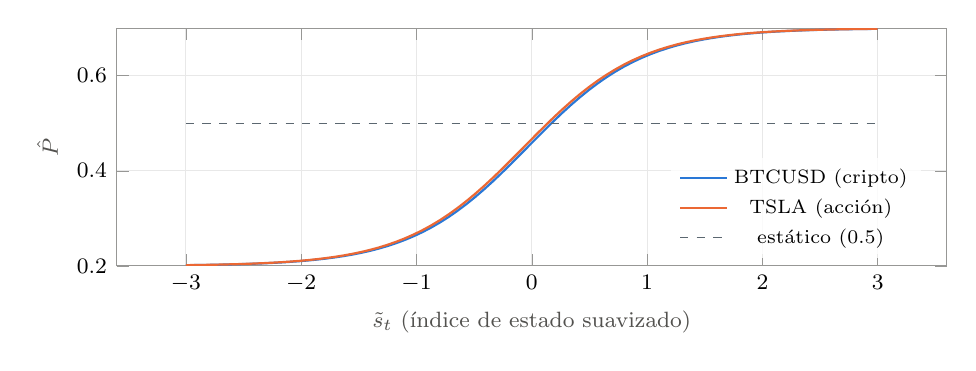
\begin{tikzpicture}\begin{axis}[estilo, ylabel={$\hat P$}, ymin=0.2, ymax=0.7, legend pos=south east]
\addplot[color=serieA, thick] {0.2+(0.7-0.2)/(1+exp(-1.97016*(x-(-0.0363374))))};\addlegendentry{BTCUSD (cripto)}
\addplot[color=serieB, thick] {0.2+(0.7-0.2)/(1+exp(-1.96965*(x-(-0.0689944))))};\addlegendentry{TSLA (acción)}
\addplot[color=cgris, dashed] {0.5};\addlegendentry{estático (0.5)}
\end{axis}\end{tikzpicture}\end{center}
\begin{center}\small\setlength{\tabcolsep}{5pt}
\begin{tabular}{llcccc}\toprule
Activo & Pesos $w_i$ & punto\_medio & pendiente & $R^2$ & Estático \\\midrule
BTCUSD & [0.10, 0.90] & -0.03634 & 1.97 & 0.968 & 0.5 \\
ETHUSD & [0.10, 0.90] & -0.0535 & 2.072 & 0.965 & 0.5 \\
TSLA & [0.10, 0.90] & -0.06899 & 1.97 & 0.911 & 0.5 \\
GOOGL & [0.10, 0.90] & -0.05139 & 2.075 & 0.900 & 0.5 \\
NVDA & [0.10, 0.90] & -0.05089 & 2.024 & 0.922 & 0.5 \\
AMZN & [0.10, 0.90] & -0.0516 & 2.064 & 0.904 & 0.5 \\
MSFT & [0.10, 0.90] & -0.06766 & 2.203 & 0.911 & 0.5 \\
\bottomrule\end{tabular}

\medskip
\begin{tabular}{lrrrr}\toprule
Activo & $\mu_1$ & $\sigma_1$ & $\mu_2$ & $\sigma_2$ \\\midrule
BTCUSD & 0.007149 & 0.003488 & 27.23 & 11.83 \\
ETHUSD & 0.009458 & 0.004748 & 27.83 & 12.14 \\
TSLA & 0.01387 & 0.004534 & 26.59 & 10.57 \\
GOOGL & 0.00848 & 0.002429 & 26.91 & 9.836 \\
NVDA & 0.01197 & 0.004393 & 26.24 & 9.885 \\
AMZN & 0.008549 & 0.003264 & 26.4 & 10.1 \\
MSFT & 0.006711 & 0.002343 & 25.47 & 10.23 \\
\bottomrule\end{tabular}\end{center}
\textbf{Lectura.} Calibra $\text{factor}_B$ solo; la interacción con $\hat A_t$ ($B$ absoluto) queda para Q5. El estático es $B/A=0.5$; el dinámico queda por debajo de él en cerca de 65\% de las barras.
\newpage
\section*{$K$ --- peso del aislamiento futuro frente al pasado}

\textbf{Qué controla.} En X0, $y=\text{Low}_{left}+\text{High}_{left}+K(\text{Low}_{right}+\text{High}_{right})$. $K$ alto premia niveles que siguieron intactos después de formarse; bajo, el contexto previo.

\textbf{Hipótesis.} Mercado estable, sin rupturas recientes $\rightarrow$ $K$ alto. Rupturas seguidas o cambios de régimen $\rightarrow$ $K$ bajo.

\textbf{Variables} (velas H1):
\begin{itemize}\setlength{\itemsep}{1pt}\setlength{\topsep}{1pt}
\item $x_1=-|\text{ruptura}_t|$, con $\text{ruptura}_t=+1$ si $C_t>\max_{i=t-20..t-1}H_i$, $-1$ si $C_t<\min_{i=t-20..t-1}L_i$ y $0$ en otro caso (canal de Donchian de 20 barras). Valor absoluto porque una ruptura al alza y una a la baja son ambas un nivel que no se sostuvo; signo invertido para que pendiente positiva signifique estabilidad.
\end{itemize}
Una variable: peso $1$. Suavizado: EMA causal con \code{span=12}.

\begin{center}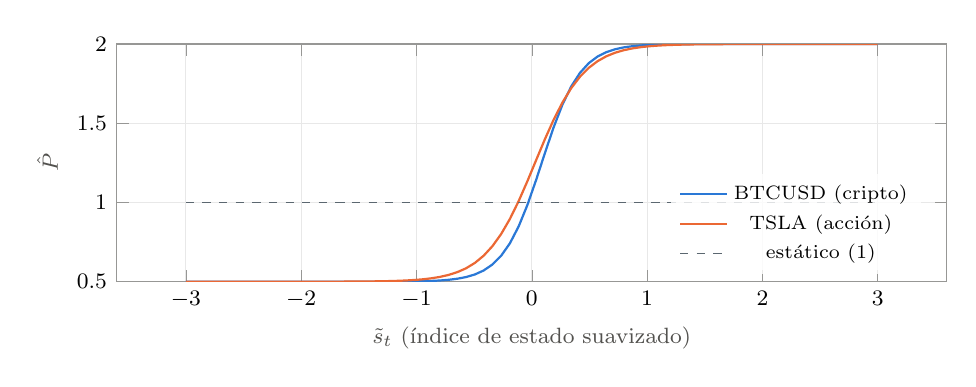
\begin{tikzpicture}\begin{axis}[estilo, ylabel={$\hat P$}, ymin=0.5, ymax=2, legend pos=south east]
\addplot[color=serieA, thick] {0.5+(2-0.5)/(1+exp(-5.96831*(x-(0.0858844))))};\addlegendentry{BTCUSD (cripto)}
\addplot[color=serieB, thick] {0.5+(2-0.5)/(1+exp(-4.70838*(x-(0.0277035))))};\addlegendentry{TSLA (acción)}
\addplot[color=cgris, dashed] {1};\addlegendentry{estático (1)}
\end{axis}\end{tikzpicture}\end{center}
\begin{center}\small\setlength{\tabcolsep}{5pt}
\begin{tabular}{llcccc}\toprule
Activo & Pesos $w_i$ & punto\_medio & pendiente & $R^2$ & Estático \\\midrule
BTCUSD & [1.00] & 0.08588 & 5.968 & 0.927 & 1 \\
ETHUSD & [1.00] & 0.05676 & 5.958 & 0.928 & 1 \\
TSLA & [1.00] & 0.0277 & 4.708 & 0.958 & 1 \\
GOOGL & [1.00] & 0.0247 & 4.845 & 0.936 & 1 \\
NVDA & [1.00] & 0.03223 & 4.888 & 0.960 & 1 \\
AMZN & [1.00] & 0.02281 & 4.709 & 0.952 & 1 \\
MSFT & [1.00] & 0.0359 & 4.963 & 0.956 & 1 \\
\bottomrule\end{tabular}

\medskip
\begin{tabular}{lrr}\toprule
Activo & $\mu_1$ & $\sigma_1$ \\\midrule
BTCUSD & -0.0828 & 0.2756 \\
ETHUSD & -0.08054 & 0.2721 \\
TSLA & -0.1347 & 0.3414 \\
GOOGL & -0.136 & 0.3427 \\
NVDA & -0.1405 & 0.3475 \\
AMZN & -0.1336 & 0.3403 \\
MSFT & -0.129 & 0.3352 \\
\bottomrule\end{tabular}\end{center}
\textbf{Lectura.} La evidencia «alta» de Q3 para \code{ruptura\_rango} (Pearson 0.50) es mecánica: se define con el cierre de la propia barra y coincide con el retorno de esa hora; con el retorno siguiente la correlación es $-0.003$. La elección descansa en la hipótesis. Es la serie menos suave de la fase: cambia en promedio 6.8\% de su rango por barra (las demás, 0.4\%--3.6\%), porque cada ruptura mueve $z$ unas 3.3 desviaciones; el \code{span} se calibra en Q5. $K$ es global en producción; aquí se calibra por activo solo como diagnóstico.
\newpage
\section*{$N_{EXP}$ --- exponente de recencia}

\textbf{Qué controla.} Peso de cada vela en la función objetivo de X0: $w=t^{N_{EXP}}$, $t\in[0,1]$ (1 = la más reciente). Alto concentra el peso en lo reciente; bajo lo reparte parejo.

\textbf{Hipótesis.} Cambio de régimen o volatilidad creciente $\rightarrow$ $N_{EXP}$ alto. Mercado estable y repetitivo $\rightarrow$ bajo.

\textbf{Variables} (velas H1):
\begin{itemize}\setlength{\itemsep}{1pt}\setlength{\topsep}{1pt}
\item $x_1=\text{cambio\_volatilidad}_t=vol_{24,t}/vol_{168,t}$, con $vol_{n,t}=\sqrt{8760}\cdot\text{std}(r_{t-n+1..t})$ y $r_t=\ln(C_t/C_{t-1})$.
\end{itemize}
Una variable: peso $1$. Suavizado: EMA causal con \code{span=12}.

\begin{center}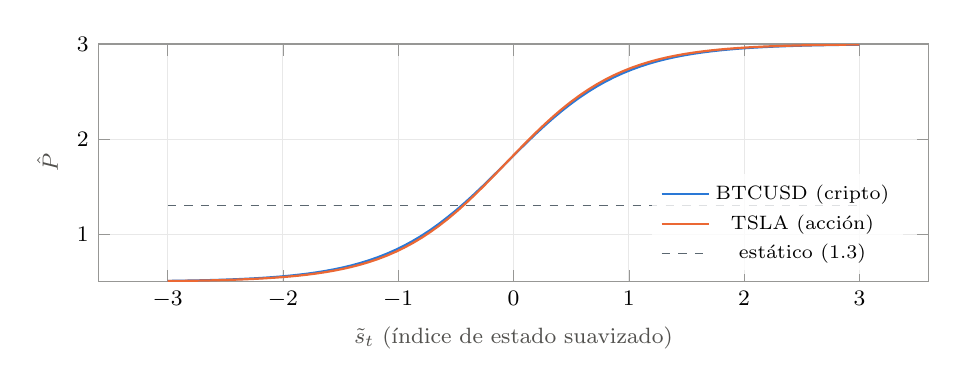
\begin{tikzpicture}\begin{axis}[estilo, ylabel={$\hat P$}, ymin=0.5, ymax=3, legend pos=south east]
\addplot[color=serieA, thick] {0.5+(3-0.5)/(1+exp(-1.94445*(x-(-0.063271))))};\addlegendentry{BTCUSD (cripto)}
\addplot[color=serieB, thick] {0.5+(3-0.5)/(1+exp(-2.02256*(x-(-0.0633857))))};\addlegendentry{TSLA (acción)}
\addplot[color=cgris, dashed] {1.3};\addlegendentry{estático (1.3)}
\end{axis}\end{tikzpicture}\end{center}
\begin{center}\small\setlength{\tabcolsep}{5pt}
\begin{tabular}{llcccc}\toprule
Activo & Pesos $w_i$ & punto\_medio & pendiente & $R^2$ & Estático \\\midrule
BTCUSD & [1.00] & -0.06327 & 1.944 & 0.988 & 1.3 \\
ETHUSD & [1.00] & -0.05559 & 1.98 & 0.986 & 1.3 \\
TSLA & [1.00] & -0.06339 & 2.023 & 0.974 & 1.3 \\
GOOGL & [1.00] & -0.08578 & 2.111 & 0.960 & 1.3 \\
NVDA & [1.00] & -0.01337 & 2.151 & 0.973 & 1.3 \\
AMZN & [1.00] & -0.06947 & 1.989 & 0.959 & 1.3 \\
MSFT & [1.00] & -0.06034 & 2.109 & 0.958 & 1.3 \\
\bottomrule\end{tabular}

\medskip
\begin{tabular}{lrr}\toprule
Activo & $\mu_1$ & $\sigma_1$ \\\midrule
BTCUSD & 0.9359 & 0.3701 \\
ETHUSD & 0.9401 & 0.3545 \\
TSLA & 0.9579 & 0.2809 \\
GOOGL & 0.9401 & 0.3503 \\
NVDA & 0.9528 & 0.2974 \\
AMZN & 0.9429 & 0.3479 \\
MSFT & 0.9496 & 0.3419 \\
\bottomrule\end{tabular}\end{center}
\textbf{Lectura.} La evidencia de Q2/Q3 para esta variable es baja ($|\rho|<0.01$); se mantiene por la hipótesis y el $R^2$ alto no la respalda (sale casi por construcción). $N_{EXP}$ es global en producción.
\newpage
\section*{$\lambda$ --- castigo por soportes desparejos}

\textbf{Qué controla.} En X0, $FO=\text{mean}(z)-\lambda\cdot cv(H_n)$, con $cv(H_n)$ el coeficiente de variación de los huecos entre soportes consecutivos. $\lambda$ alto empuja a repartirlos parejo; bajo, a concentrarlos donde hay más evidencia.

\textbf{Hipótesis.} Rango amplio y lateral con soportes concentrados $\rightarrow$ $\lambda$ alto.

\textbf{Variables} (velas H1):
\begin{itemize}\setlength{\itemsep}{1pt}\setlength{\topsep}{1pt}
\item $x_1=\text{bb\_width}_t=4\sigma_t/\mu_t$: ancho de bandas de Bollinger (ventana 20, $k=2$).
\item $x_2=\text{duracion\_en\_rango}_t$: barras desde la última ruptura del canal de 20 barras (contador que se reinicia a 0).
\end{itemize}
Peso $w_1$ por grilla y mejor $R^2$: $[0.2,\,0.8]$ o $[0.3,\,0.7]$ (domina la duración en rango). Suavizado: EMA causal con \code{span=12}.

\begin{center}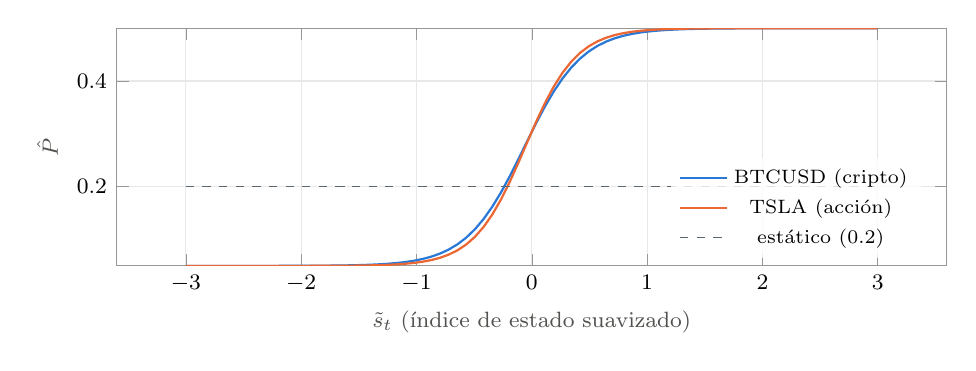
\begin{tikzpicture}\begin{axis}[estilo, ylabel={$\hat P$}, ymin=0.05, ymax=0.5, legend pos=south east]
\addplot[color=serieA, thick] {0.05+(0.5-0.05)/(1+exp(-3.97485*(x-(-0.0650854))))};\addlegendentry{BTCUSD (cripto)}
\addplot[color=serieB, thick] {0.05+(0.5-0.05)/(1+exp(-4.5254*(x-(-0.0579431))))};\addlegendentry{TSLA (acción)}
\addplot[color=cgris, dashed] {0.2};\addlegendentry{estático (0.2)}
\end{axis}\end{tikzpicture}\end{center}
\begin{center}\small\setlength{\tabcolsep}{5pt}
\begin{tabular}{llcccc}\toprule
Activo & Pesos $w_i$ & punto\_medio & pendiente & $R^2$ & Estático \\\midrule
BTCUSD & [0.20, 0.80] & -0.06509 & 3.975 & 0.966 & 0.2 \\
ETHUSD & [0.20, 0.80] & -0.1344 & 4.463 & 0.971 & 0.2 \\
TSLA & [0.30, 0.70] & -0.05794 & 4.525 & 0.965 & 0.2 \\
GOOGL & [0.20, 0.80] & -0.1042 & 4.171 & 0.964 & 0.2 \\
NVDA & [0.30, 0.70] & -0.03401 & 4.832 & 0.966 & 0.2 \\
AMZN & [0.20, 0.80] & -0.1098 & 4.337 & 0.965 & 0.2 \\
MSFT & [0.20, 0.80] & -0.1174 & 4.583 & 0.968 & 0.2 \\
\bottomrule\end{tabular}

\medskip
\begin{tabular}{lrrrr}\toprule
Activo & $\mu_1$ & $\sigma_1$ & $\mu_2$ & $\sigma_2$ \\\midrule
BTCUSD & 0.03029 & 0.02424 & 13.34 & 13.08 \\
ETHUSD & 0.04075 & 0.03261 & 13.32 & 13.08 \\
TSLA & 0.07291 & 0.04212 & 8.936 & 9.12 \\
GOOGL & 0.04838 & 0.02882 & 7.764 & 7.489 \\
NVDA & 0.06215 & 0.03908 & 8.357 & 8.272 \\
AMZN & 0.04385 & 0.0305 & 8.471 & 8.608 \\
MSFT & 0.03407 & 0.02253 & 9.109 & 9.156 \\
\bottomrule\end{tabular}\end{center}
\textbf{Lectura.} Rango $(0.05,\,0.5)$ definido por Mauricio el 2026-11-02 para contener el valor productivo $0.2$; el rango documentado $(0.001,\,0.02)$ lo dejaba fuera. Evidencia de Q3 baja para ambas variables. La duración en rango es un contador de dientes de sierra, así que $\hat\lambda_t$ es la segunda serie menos suave (3.6\% del rango por barra). Global en producción.
\newpage
\section*{$\text{PERDIDA\_MAX}$ --- pérdida tolerada por posición}

\textbf{Qué controla.} Si la pérdida flotante $(P_i-P_0)\cdot L$ de una posición supera este umbral en USD, X1 la cierra a mercado, sin importar el trailing. Escala con el lotaje real.

\textbf{Hipótesis.} Drawdown de 7 días sano $\rightarrow$ umbral alto (hay más chance de recuperación). Drawdown profundo $\rightarrow$ umbral bajo (la caída tiende a continuar).

\textbf{Variables} (velas H1):
\begin{itemize}\setlength{\itemsep}{1pt}\setlength{\topsep}{1pt}
\item $x_1=\text{drawdown}_{7d}=(C_t-M_t)/M_t$, con $M_t=\max_{i=t-167..t}C_i$ (168 barras H1 = 7 días). Elegida por ser la variable de evidencia alta y estable en los 7 activos de Q2 (Pearson medio $+0.115$ con el retorno de la hora siguiente) que no usa $N$.
\end{itemize}
Una variable: peso $1$. Suavizado: EMA causal con \code{span=12}.

\begin{center}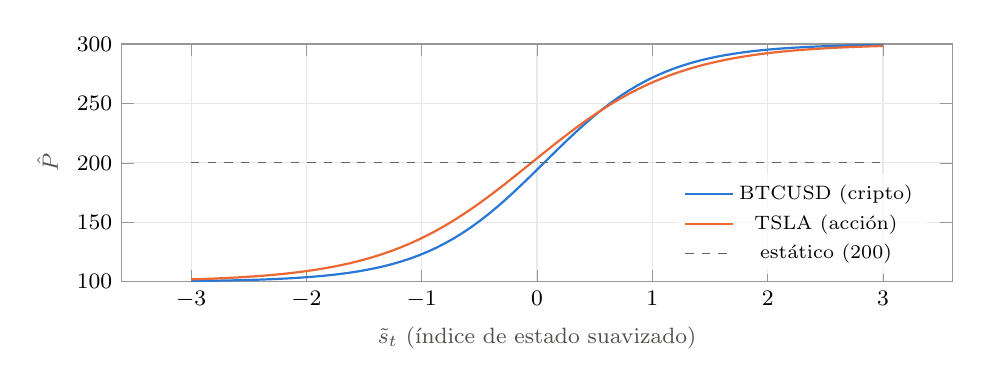
\begin{tikzpicture}\begin{axis}[estilo, ylabel={$\hat P$}, ymin=100, ymax=300, legend pos=south east]
\addplot[color=serieA, thick] {100+(300-100)/(1+exp(-1.91876*(x-(0.0600188))))};\addlegendentry{BTCUSD (cripto)}
\addplot[color=serieB, thick] {100+(300-100)/(1+exp(-1.57022*(x-(-0.0491824))))};\addlegendentry{TSLA (acción)}
\addplot[color=cgris, dashed] {200};\addlegendentry{estático (200)}
\end{axis}\end{tikzpicture}\end{center}
\begin{center}\small\setlength{\tabcolsep}{5pt}
\begin{tabular}{llcccc}\toprule
Activo & Pesos $w_i$ & punto\_medio & pendiente & $R^2$ & Estático \\\midrule
BTCUSD & [1.00] & 0.06002 & 1.919 & 0.887 & 200 \\
ETHUSD & [1.00] & 0.1478 & 1.976 & 0.900 & 200 \\
TSLA & [1.00] & -0.04918 & 1.57 & 0.917 & 200 \\
GOOGL & [1.00] & -0.09354 & 1.47 & 0.868 & 200 \\
NVDA & [1.00] & -0.07883 & 1.447 & 0.802 & 200 \\
AMZN & [1.00] & 0.01814 & 1.57 & 0.818 & 200 \\
MSFT & [1.00] & -0.02204 & 1.617 & 0.878 & 200 \\
\bottomrule\end{tabular}

\medskip
\begin{tabular}{lrr}\toprule
Activo & $\mu_1$ & $\sigma_1$ \\\midrule
BTCUSD & -0.04231 & 0.04128 \\
ETHUSD & -0.05802 & 0.05571 \\
TSLA & -0.09603 & 0.07903 \\
GOOGL & -0.05548 & 0.04825 \\
NVDA & -0.06895 & 0.0658 \\
AMZN & -0.0561 & 0.05524 \\
MSFT & -0.04337 & 0.03933 \\
\bottomrule\end{tabular}\end{center}
\textbf{Lectura.} La evidencia es contra el retorno del activo, no contra la pérdida adversa de una posición. \code{x5\_contexto\_conversacion.md} §10 dejó este parámetro pausado por si pasa a una capa externa de riesgo.
\end{document}
